\section{A list is a sequence}
\label{sequence}

Like a string, a \textbf{list} is a sequence of values. In a string, the values are characters; in a list, they can be of any type. Values in a list are called \textbf{items}.
\index{lista}
\index{tipo!lista}
\index{elemento}
\index{secuencia}
\index{item@ítem}

There are several ways to create a new list; the simplest is to enclose the elements in square brackets (\verb"[" and \verb"]"):

\begin{Verbatim}[frame=single]
[10, 20, 30, 40]
['crunchy frog', 'ram bladder', 'lark vomit']
\end{Verbatim}
%
The first example is a list of four integers. The second is a list of three strings. The elements of a list do not necessarily have to be of the same type. The following list contains a string, a floating point number, an integer, and (note!) another list:

\begin{Verbatim}[frame=single]
['spam', 2.0, 5, [10, 20]]
\end{Verbatim}
%
A list within another list is \textbf{nested}.
\index{lista!anidada}
\index{anidada, lista}

A list that contains no elements is called an empty list; you can create one with empty square brackets, \verb"[]".
\index{lista!vacía}
\index{vacía!lista}

As you might expect, you can assign list values to variables:

\begin{Verbatim}[frame=single]
>>> cheeses = ['Cheddar', 'Edam', 'Gouda']
>>> numbers = [42, 123]
>>> empty = []
>>> print(cheeses, numbers, empty)
['Cheddar', 'Edam', 'Gouda'] [42, 123] []
\end{Verbatim}
%
\index{asignación}


\section{Lists are mutable}
\label{mutable}
\index{lista!elemento}
\index{acceso}
\index{indice@índice}
\index{operador!de corchetes}
\index{corchetes!operador de}

The syntax for accessing elements of a list is the same as for accessing characters in a string: the bracket operator. The expression inside the brackets specifies the index. Remember that indices start at 0:

\begin{Verbatim}[frame=single]
>>> cheeses[0]
'Cheddar'
\end{Verbatim}
%
Unlike strings, lists are mutable. When the bracket operator appears on the left side of an assignment, it identifies the list item to be assigned.
\index{mutabilidad}

\begin{Verbatim}[frame=single]
>>> numbers = [42, 123]
>>> numbers[1] = 5
>>> numbers
[42, 5]
\end{Verbatim}
%
The one-th element of \texttt{numbers}, which used to be 123, is now 5.
\index{indice@índice!comenzando en cero}
\index{cero, índice comenzando en}

Figure~\ref{fig.liststate} shows the state diagram for {\tt
cheeses}, \texttt{numbers} and \texttt{empty}.
\index{diagrama!de estado}
\index{estado, diagrama de}

\begin{figure}
\centerline
{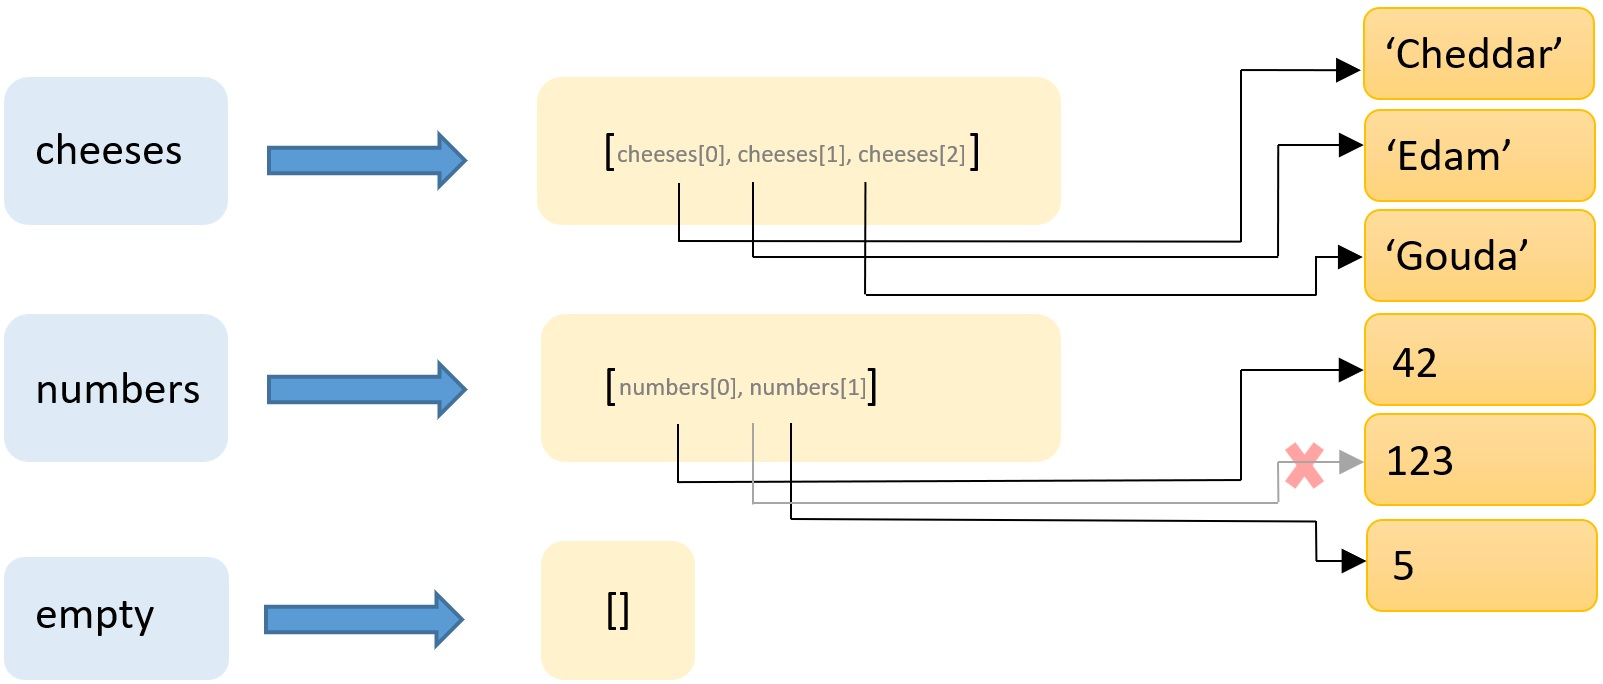
\includegraphics[scale=0.45]{images/state-diagram.jpg}}
\caption{State diagram}
\label{fig.liststate}
\end{figure}

Lists are represented by boxes with the word ``list'' on the outside and the elements of the list inside. \texttt{cheese} refers to a list with three elements with indices 0, 1 and 2. \texttt{numbers} contains two elements; the diagram shows that the value of the second element has been reassigned from 123 to 5. \texttt{empty} refers to a list with no elements.
\index{asignación de ítem}
\index{item@ítem!asignación de}
\index{reasignación}

List indices work the same way as string indices:

\begin{itemize}

\item Any integer expression can be used as an index.

\item If you try to read or write an element that doesn't exist, you get an \texttt{IndexError}.
\index{excepción!IndexError}
\index{IndexError}

\item If an index has a negative value, it is counted down from the end of the list.

\end{itemize}
\index{lista!indice de@índice de}

\index{lista!pertenencia}
\index{pertenencia!lista}
\index{operador!in}
\index{in, operador}

The \texttt{in} operator also works on lists.

\begin{Verbatim}[frame=single]
>>> cheeses = ['Cheddar', 'Edam', 'Gouda']
>>> 'Edam' in cheeses
True
>>> 'Brie' in cheeses
False
\end{Verbatim}


\section{Looping through a list}
\index{recorrer!lista}
\index{lista!recorrer}
\index{bucle!for}
\index{for, bucle}
\index{sentencia!for}

The most common way to iterate through the elements of a list is with a \texttt{for} loop. The syntax is the same as for strings:

\begin{Verbatim}[frame=single]
for cheese in cheeses:
    print(cheese)
\end{Verbatim}
%
This works fine if you only need to read the elements of the list. But if you want to write or update the elements, you need the indexes. A common way to do this is to combine the \texttt{range} and \texttt{len} built-in functions:
\index{bucle!con índices}
\index{indice@índice!bucle con}

\begin{python}[frame=single]
for i in range(len(numbers)):
    numbers[i] = numbers[i] * 2
\end{python}
%
This loop iterates through the elements of the list and updates each of them. \texttt{len} returns the number of elements in the list. \texttt{range} returns a list of indices from 0 to $n-1$, where $n$ is the length of the list. At each iteration through the loop, \texttt{i} gets the index of the next element. The assignment statement in the body uses \texttt{i} to read the old value of the element and assign the new value.
\index{actualizar!item@ítem}
\index{item@ítem!actualizar}

A \texttt{for} loop through an empty list never executes the body:

\begin{python}[frame=single]
for x in []:
    print('This never happens.')
\end{python}
%
Even though a list can contain another list, the nested list still counts as a single element. The length of this list is four:
\index{lista!anidada}
\index{anidada, lista}

\begin{Verbatim}[frame=single]
['spam', 1, ['Brie', 'Roquefort', 'Pol le Veq'], [1, 2, 3]]
\end{Verbatim}



\section{List operations}
\index{lista!operación}

The \texttt{+} operator concatenates lists:
\index{lista!concatenación}
\index{concatenación!lista}

\begin{Verbatim}[frame=single]
>>> a = [1, 2, 3]
>>> b = [4, 5, 6]
>>> c = a + b
>>> c
[1, 2, 3, 4, 5, 6]
\end{Verbatim}
%
The \texttt{*} operator repeats a list a given number of times:
\index{repetición!lista}
\index{lista!repetición}

\begin{Verbatim}[frame=single]
>>> [0] * 4
[0, 0, 0, 0]
>>> [1, 2, 3] * 3
[1, 2, 3, 1, 2, 3, 1, 2, 3]
\end{Verbatim}
%
The first example repeats \texttt{[0]} four times. The second example repeats the list \texttt{[1, 2, 3]} three times.


\section{List slices}
\index{operador!de trozo}
\index{trozo!operador}
\index{indice@índice!de trozo}
\index{lista!trozo}
\index{trozo!lista}\index{slice}

The slice operator that we have seen for strings also works on lists:

\begin{Verbatim}[frame=single]
>>> t = ['a', 'b', 'c', 'd', 'e', 'f']
>>> t[1:3]
['b', 'c']
>>> t[:4]
['a', 'b', 'c', 'd']
>>> t[3:]
['d', 'e', 'f']
\end{Verbatim}
%
If you omit the first index, the chunk starts at the beginning. If you omit the second, the chunk goes to the end. So if you omit both, the chunk is a copy of the entire list.
\index{lista!copia}
\index{trozo!copia de}
\index{copia!de trozo}

\begin{Verbatim}[frame=single]
>>> t[:]
['a', 'b', 'c', 'd', 'e', 'f']
\end{Verbatim}
%
Since lists are mutable, it is often useful to create a copy before performing operations that modify lists.
\index{mutabilidad}

A slice operator on the left side of an assignment can update multiple elements:
\index{trozo!actualizar}\index{slice}
\index{actualizar!trozo}

\begin{Verbatim}[frame=single]
>>> t = ['a', 'b', 'c', 'd', 'e', 'f']
>>> t[1:3] = ['x', 'y']
>>> t
['a', 'x', 'y', 'd', 'e', 'f']
\end{Verbatim}
%

% You can add elements to a list by squeezing them into an empty
% slice:

% % \begin{Verbatim}[frame=single]
% >>> t = ['a', 'd', 'e', 'f']
% >>> t[1:1] = ['b', 'c']
% >>> print t
% ['a', 'b', 'c', 'd', 'e', 'f']
% \end{Verbatim}
% \afterverb
%
% And you can remove elements from a list by assigning the empty list to
% them:

% % \begin{Verbatim}[frame=single]
% >>> t = ['a', 'b', 'c', 'd', 'e', 'f']
% >>> t[1:3] = []
% >>> print t
% ['a', 'd', 'e', 'f']
% \end{Verbatim}
% \afterverb
%
% But both of those operations can be expressed more clearly
% with list methods.


\section{List methods}
\index{lista!método de}
\index{metodo@método!de lista}

Python provides methods that operate on lists. Methods are called with the dot notation, as we will see in the example below that uses \pythoninline{t.append('d')}. For example, \texttt{append} adds a new element to the end of the list: \index{method@method!append}
\index{append, método}

\begin{Verbatim}[frame=single]
>>> t = ['a', 'b', 'c']
>>> t.append('d')
>>> t
['a', 'b', 'c', 'd']
\end{Verbatim}



\texttt{extend} takes another list as an argument and appends all the elements:
\index{metodo@método!extend}
\index{extend, método}

\begin{Verbatim}[frame=single]
>>> t1 = ['a', 'b', 'c']
>>> t2 = ['d', 'e']
>>> t1.extend(t2)
>>> t1
['a', 'b', 'c', 'd', 'e']
\end{Verbatim}
%
This example leaves \texttt{t2} unchanged.

\texttt{sort} sorts the elements of the list from smallest to largest:
\index{metodo@método!sort}
\index{sort, método}

\begin{Verbatim}[frame=single]
>>> t = ['d', 'c', 'e', 'b', 'a']
>>> t.sort()
>>> t
['a', 'b', 'c', 'd', 'e']
\end{Verbatim}
%
Most list methods are null: they modify the list and return \texttt{None}. If you write \texttt{t = t.sort()}, you will be disappointed with the result.
\index{metodo@método!nulo}
\index{nulo, método}
\index{valor especial!None}
\index{None, valor especial}


\section{Going through lists}
\label{filter}

To add all the numbers in a list, you can use a loop like this:

\begin{python}[frame=single]
def add_all(t):
    total = 0
    for x in t:
        total += x
    return total
\end{python}

\index{operador!de actualización}
\index{actualización, operador de}
\index{aumentada, asignación}
\index{asignación!aumentada}

\texttt{total} is initialized to 0. On each pass through the loop, \texttt{x} gets an element from the list. Remember that the \pythoninline{+=} operator provides a shorthand way to update a variable. This \textbf{augmented assignment statement}:

\begin{Verbatim}[frame=single]
total += x
\end{Verbatim}
%
It is equivalent to

\begin{Verbatim}[frame=single]
total = total + x
\end{Verbatim}
%
As the loop executes, \pythoninline{total} accumulates the sum of the elements; a variable used in this way is sometimes called a \textbf{ accumulator}.
\index{acumulador de suma}

Adding the elements of a list is such a common operation that Python provides it as a built-in function, \pythoninline{sum}:

\begin{Verbatim}[frame=single]
>>> t = [1, 2, 3]
>>> sum(t)
6
\end{Verbatim}
%
An operation like this that combines a sequence of elements into a single value is sometimes called \textbf{reduction}.
\index{patrón!de reducción}
\index{reducción, patrón de}
\index{recorrer}

Sometimes you want to loop through one list while building another. For example, the following function takes a list of strings and returns a new list containing strings that start with a capital letter:

\begin{python}[frame=single]
def all_with_capital_letter(t):
    res = []
    for s in t:
        res.append(s.capitalize())
    return res
\end{python}
%
The variable \pythoninline{res} is initialized to an empty list; at each pass through the loop, we append the next element. So \pythoninline{res} is another type of accumulator.
\index{acumulador lista}

A traversal like the one in \pythoninline{all_with_capital_letter} is sometimes called \textbf{map} because it ``maps'' a function (in this case the \pythoninline{capitalize} method) over each of the elements in a sequence.
\index{patrón!de mapa}
\index{mapa, patrón de}
\index{patrón!de filtro}
\index{filtro, patrón de}

Another common operation is to select some of the elements of a list and return a sublist. For example, the following function takes a list of strings and returns a list containing only strings written in uppercase:

\begin{python}[frame=single]
def uppercase_only(t):
    res = []
    for s in t:
        if s.isupper():
            res.append(s)
    return res
\end{python}
%
\pythoninline{isupper} is a string method that returns \pythoninline{True} if the string contains only uppercase letters.

A traversal like the one in \pythoninline{uppercase_only} is called a \textbf{filter} because it selects some of the elements and filters the others.

Most list operations can be expressed as a combination of map, filter, and reduce.


\section{Removing elements}
\index{eliminación de elementos}
\index{elemento!eliminación}

There are several ways to remove items from a list. If you know the index of the element, you can use the \pythoninline{pop} method:
\index{metodo@método!pop}
\index{pop, método}

\begin{Verbatim}[frame=single]
>>> t = ['a', 'b', 'c']
>>> x = t.pop(1)
>>> t
['a', 'c']
>>> x
'b'
\end{Verbatim}
%
\pythoninline{pop} modifies the list and returns the element that was removed.
If you don't supply an index, it removes and returns the last element.

If you don't need the removed value, you can use the \pythoninline{del} operator:
\index{operador!del}
\index{del, operador}

\begin{Verbatim}[frame=single]
>>> t = ['a', 'b', 'c']
>>> del t[1]
>>> t
['a', 'c']
\end{Verbatim}
%
If you know the element you want to remove (but not the index), you can use the \pythoninline{remove} method:
\index{metodo@método!remove}
\index{remove, método}

\begin{Verbatim}[frame=single]
>>> t = ['a', 'b', 'c']
>>> t.remove('b')
>>> t
['a', 'c']
\end{Verbatim}
%
The return value of \pythoninline{remove} is \pythoninline{None}.
\index{valor especial!None}
\index{None, valor especial}

To remove more than one element, you can use \pythoninline{del} with slice indices:

\begin{Verbatim}[frame=single]
>>> t = ['a', 'b', 'c', 'd', 'e', 'f']
>>> del t[1:5]
>>> t
['a', 'f']
\end{Verbatim}
%
As usual, the slice selects all elements up to but not including the second index.


\section{Lists and strings}
\index{lista}
\index{cadena}
\index{secuencia}

A string is a sequence of characters and a list is a sequence of values, but a list of characters is not the same as a string. To convert a string to a list of characters, you can use the \pythoninline{list} function:
\index{list, función}
\index{función!list}

\begin{Verbatim}[frame=single]
>>> s = 'spam'
>>> t = list(s)
>>> t
['s', 'p', 'a', 'm']
\end{Verbatim}
%
Since \pythoninline{list} is the name of a built-in function, you should avoid using it as a variable name. It is also good practice to avoid the letter \pythoninline{l} because it closely resembles the number \pythoninline{1}. So that's why we use \pythoninline{t} here.

The \pythoninline{list} function breaks the string into individual letters. If you want to split a string into words, you can use the \pythoninline{split} method:
\index{metodo@método!split}
\index{split, método}

\begin{Verbatim}[frame=single]
>>> s = 'pining for the fjords'
>>> t = s.split()
>>> t
['pining', 'for', 'the', 'fjords']
\end{Verbatim}
%
An optional argument called \textbf{delimiter} specifies which characters to use as the word separator. The following example uses a hyphen as a delimiter:
\index{argumento opcional}
\index{opcional!argumento}
\index{delimitador}

\begin{Verbatim}[frame=single]
>>> s = 'spam-spam-spam'
>>> delimiter = '-'
>>> t = s.split(delimiter)
>>> t
['spam', 'spam', 'spam']
\end{Verbatim}
%
\pythoninline{join} is the inverse of \pythoninline{split}. It takes a list of strings and concatenates the elements. \pythoninline{join} is a string method, so you have to call it on the delimiter and pass it the list as a parameter:
\index{metodo@método!join}
\index{join, método}
\index{concatenación}

\begin{Verbatim}[frame=single]
>>> t = ['pining', 'for', 'the', 'fjords']
>>> delimiter = ' '
>>> s = delimiter.join(t)
>>> s
'pining for the fjords'
\end{Verbatim}
%
In this case the delimiter is a space character, so \pythoninline{join} puts a space between the words. To concatenate strings without spaces, you can use the empty string, \verb"''", as a delimiter.
\index{cadena!vacía}
\index{vacía!cadena}


\section{Objects, values and equality}
\label{equivalence}
\index{objeto}
\index{valor}

If we run these assignment statements:

\begin{python}[frame=single]
a = 'banana'
b = 'banana'
\end{python}
%
we know that the variables \pythoninline{a} and \pythoninline{b} refer to a string, but we don't know if they refer to the {\em same} string. There are two possible states, shown in Figure~\ref{fig.list1}.
\index{alias}

\begin{figure}
\centerline
{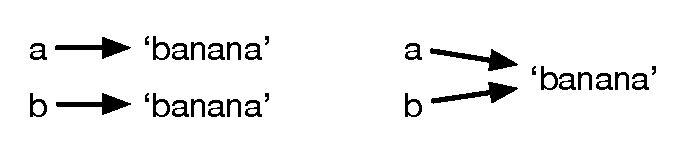
\includegraphics[scale=0.8]{images/list1.eps}}
\caption{Variables and their references to values}
\label{fig.list1}
\end{figure}

In the first case, \texttt{a} and \texttt{b} refer to two different objects that have the same value. In the second case, they refer to the same object.
\index{operador!is}
\index{is, operador}

To check if two variables refer to the same object, you can use the \pythoninline{is} operator.

\begin{Verbatim}[frame=single]
>>> a = 'banana'
>>> b = 'banana'
>>> a is b
True
>>> a == b
True
\end{Verbatim}
%
In this example, Python only creates a string object, and both \pythoninline{a} and \pythoninline{b} refer to it. But when you create two lists, Python does it differently and gives us two objects:

\begin{Verbatim}[frame=single]
>>> a = [1, 2, 3]
>>> b = [1, 2, 3]
>>> a is b
False
>>> a == b 
True
\end{Verbatim}
%


In this case we would say that the two lists are \textbf{equivalent}, because they have the same elements, but not \textbf{identical}, because they are not the same object. If two objects are identical, they are also equivalent, but if they are equivalent, they are not necessarily identical.
\index{equivalencia}
\index{identidad}

So far, we've been using ``object'' and ``value'' interchangeably, but it's more accurate to say that an object has a value. If you evaluate \pythoninline{[1, 2, 3]}, you get a list object whose value is a sequence of integers. If another list has the same elements, we say that it has the same value, but it is not the same object.
\index{objeto}
\index{valor}


\section{Alias}
\index{alias}
\index{referencia!alias}

If \texttt{a} refers to an object and you assign \texttt{b = a}, then both variables refer to the same object:

\begin{Verbatim}[frame=single]
>>> a = [1, 2, 3]
>>> b = a
>>> b is a
True
\end{Verbatim}
%

The association of a variable with an object is called \textbf{reference}. In this example, there are two references to the same object.
\index{referencia}

An object with more than one reference has more than one name, so we say that the object has an \textbf{alias}.
\index{mutabilidad}

If the aliased object is mutable, changes made with one alias affect the other:

\begin{Verbatim}[frame=single]
>>> a = [1, 2, 3]
>>> b = a
>>> b[0] = 42
>>> a
[42, 2, 3]
\end{Verbatim}
%
Although this behavior can be useful, it is error prone. In general, it's safer to avoid aliases when working with mutable objects.
\index{inmutabilidad}

For immutable objects like strings, aliases aren't that much of a problem. In this example:

\begin{Verbatim}[frame=single]
a = 'banana'
b = 'banana'
\end{Verbatim}
%
it almost never makes a difference whether \texttt{a} and \texttt{b} refer to the same string or not.


\section{List arguments}
\label{list.arguments}
\index{lista!como argumento}
\index{argumento}
\index{argumento de lista}
\index{referencia}
\index{parámetro}

When you pass a list as an argument to a function, the function gets a reference to the list. If the function modifies the list, the calling statement sees the change. For example, \pythoninline{headless} removes the first element of a list:

\begin{python}[frame=single]
def headless(t):
    del t[0]
\end{python}
%
It is used as follows:

\begin{Verbatim}[frame=single]
>>> letters = ['a', 'b', 'c']
>>> headless(letters)
>>> letters
['b', 'c']
\end{Verbatim}
%
The parameter \pythoninline{t} and the variable \pythoninline{letters} are aliases for the same object.

It is important to distinguish between operations that modify lists and operations that create new lists. For example, the \texttt{append} method modifies a list, but the \texttt{+} operator creates a new list.
\index{metodo@método!append}
\index{append, método}
\index{lista!concatenación}
\index{concatenación!lista}

Here's an example that uses \texttt{append}:
%
\begin{Verbatim}[frame=single]
>>> t1 = [1, 2]
>>> t2 = t1.append(3)
>>> t1
[1, 2, 3]
>>> t2
None
\end{Verbatim}
%
The return value of \texttt{append} is \texttt{None}.

Here is an example that uses the \texttt{+} operator:
%
\begin{Verbatim}[frame=single]
>>> t3 = t1 + [4]
>>> t1
[1, 2, 3]
>>> t3
[1, 2, 3, 4]
\end{Verbatim}
%
The result of when using the operator is a new list and the original list has not changed.

This difference is important when you write functions that are supposed to modify lists. For example, this function {\em DOES NOT} remove the head of a list:
%
\begin{python}[frame=single]
def wrong_headless(t):
    t = t[1:]              
\end{python}
%
The slice operator creates a new list and the assignment causes \pythoninline{t} to refer to it, but that doesn't affect the caller.
\index{operador!de trozo}\index{slice}
\index{trozo!operador}
%
\begin{Verbatim}[frame=single]
>>> t4 = [1, 2, 3]
>>> wrong_headless(t4)
>>> t4
[1, 2, 3]
\end{Verbatim}
%
At the beginning of \pythoninline{wrong_headless}, \pythoninline{t} and \pythoninline{t4} refer to the same list. At the end, \pythoninline{t} refers to a new list, but \pythoninline{t4} still refers to the original, unmodified list.

An alternative is to write a function that creates and returns a new list. For example, \pythoninline{queue} returns all elements of a list except the first:

\begin{python}[frame=single]
def queue(t):
    return t[1:]
\end{python}
%
This function leaves the original list unchanged.
It is used as follows:

\begin{Verbatim}[frame=single]
>>> letters = ['a', 'b', 'c']
>>> remainder = cola(letters)
>>> remainder
['b', 'c']
\end{Verbatim}



\section{Debugging}
\index{depuración}

Careless use of lists (and other mutable objects) can lead to long hours of debugging. Here are some common errors and ways to avoid them:

\begin{enumerate}

\item Most list methods modify the argument and return \pythoninline{None}. This is the opposite of string methods, which return a new string and leave the original as it is.

If you got used to writing chain code like this:

\begin{python}[frame=single]
word = word.strip()
\end{python}

It's tempting to write list code like this:

\begin{python}[frame=single]
t = t.sort()           
\end{python}
\index{metodo@método!sort}
\index{sort, método}

But since \pythoninline{sort} returns \pythoninline{None}, the next operation you do with \pythoninline{t} is likely to fail.

Before using list methods and operators, you should read the documentation carefully and then test them in interactive mode.

\item Choose one way and continue with that.

Part of the problem with lists is that there are so many ways to do things. For example, to remove an element from a list, you can use \pythoninline{pop}, \pythoninline{remove}, \pythoninline{del}, or even a chunk assignment.

To add an element, you can use the \pythoninline{append} method or the pythoninline \texttt{+} method. Assuming \pythoninline{t} is a list and \pythoninline{x} is a list element, these lines are correct:

\begin{Verbatim}[frame=single]
t.append(x)
t = t + [x]
t += [x]
\end{Verbatim}

And these are wrong:

\begin{Verbatim}[frame=single]
t.append([x])          # WRONG!
t = t.append(x)        # WRONG!
t + [x]                # WRONG!
t = t + x              # WRONG!
\end{Verbatim}

Try each of these examples in interactive mode to make sure you understand what you're doing. Note that only the last one causes a runtime error; the other three are legal, but do the wrong thing.


\item Create copies to avoid aliases.
\index{alias!copiar para evitar}
\index{copia!para evitar alias}

If you want to use a method like \pythoninline{sort} that modifies the argument, but you need to keep the original list as well, you can create a copy.

\begin{Verbatim}[frame=single]
>>> t = [3, 1, 2]
>>> t2 = t[:]
>>> t2.sort()
>>> t
[3, 1, 2]
>>> t2
[1, 2, 3]
\end{Verbatim}

In this example you could also use the \pythoninline{sorted} builtin function, which returns a new sorted list and leaves the original one as it is.
\index{sorted, función}
\index{función!sorted}

\begin{Verbatim}[frame=single]
>>> t2 = sorted(t)
>>> t
[3, 1, 2]
>>> t2
[1, 2, 3]
\end{Verbatim}

\end{enumerate}



\section{Glossary}

\begin{description}

\item[alias:] A circumstance where two or more variables refer to the same object.
\index{alias}

\item[accumulator:] A variable used in a loop to add or accumulate a result.
\index{acumulador}

\item[augmented assignment statement:] A statement that updates the value of a variable using an operator such as \verb"+=".
\index{aumentada, asignación}
\index{asignación aumentada}
\index{recorrer}

\item[delimiter:] A character or string used to indicate where a string should be separated.
\index{delimitador}

\item[element:] One of the values in a list (or other sequence), also called items.
\index{elemento}

\item[equivalent:] Which has the same value.
\index{equivalencia}

\item[filter:] A processing pattern that iterates through a list and selects the elements that satisfy some criteria.
\index{patrón!de filtro}
\index{filtro, patrón de}

\item[identical:] Which is the same object (which implies equivalence).
\index{identidad}

\item[list:] A sequence of values.
\index{lista}

\item[map:] A processing pattern that iterates through a sequence and performs an operation on each element.
\index{patrón!de mapa}
\index{mapa, patrón de}

\item[nested list:] A list that is an element of another list.
\index{lista!anidada}

\item[object:] Something to which a variable can refer. An object has a type and a value.
\index{objeto}

\item[reduction:] A processing pattern that iterates through a sequence and accumulates the elements into a single result.
\index{patrón!de reducción}
\index{reducción, patrón de}

\item[reference:] The association between a variable and its value.
\index{referencia}

\end{description}


\section*{Exercises}
\addcontentsline{toc}{section}{Exercises}

\begin{exercise}
Write a \pythoninline{stuff\_with\_lists} module that has the following functions with their respective pytests.

\begin{itemize}
\item A function (\pythoninline{sum_list}) to sum all elements in the list (without using the \pythoninline{sum} built-in function)
\item A function (\pythoninline{mult_list}) to multiply all elements in the list.
\item A function (\pythoninline{max_list}) to get the maximum number of the list (without using the \pythoninline{max} built-in function)
\item A function (\pythoninline{min_list}) to get the minimum number of the list (without using the \pythoninline{min} built-in function)
\end{itemize}

Your functions have to pass the following tests:\\

\begin{small}
\begin{python}
@pytest.mark.parametrize("testcase, input, expected_output",[
(1, [0,2,3,0,6,8], 19),         #sum with 0
(2, [0], 0),                    #only 1 element
(3, [], 0)])                    #empty list

def test_sum_list(testcase, input, expected_output):
    assert sum_list(input) == expected_output,\
           "case {0}".format(testcase)
    
@pytest.mark.parametrize("testcase, input, expected_output",[
(1, [0,2,3,0,6,8], 0),          #list with number 0
(2, [1,2,3,6], 36),             #list without number 0
(3, [1], 1),                    #only 1 element
(4, [], "undefined")])          #empty list

def test_mult_list(testcase, input, expected_output):
    assert mult_list(input) == expected_output,\
           "case {0}".format(testcase)
    
@pytest.mark.parametrize("testcase, input, expected_output",[
(1, [0,2,3,0,6,8], 8),          #max at the end
(2, [8,2,3,0], 8),              #max at the beginning
(3, [2,8,3,0], 8),              #max not at the beginning nor at the end
(4, [8,2,8,3,0], 8),            #max it's repeated
(5, [1,2,3,-6], 3),             #negative numbers
(6, [1], 1),                    #only 1 element
(7, [], "undefined")])          #empty list

def test_max_list(testcase, input, expected_output):
    assert max_num_in_list(input) == expected_output,\
           "case {0}".format(testcase)
 
@pytest.mark.parametrize("testcase, input, expected_output",[
(1, [1,2,3,6,8,0], 0),   #min at the end
(2, [0,8,2,3], 0),       #min at the beginning
(3, [2,8,1,5,3], 1),     #min not at the beginning nor at the end
(4, [8,0,2,3,0], 0),     #min it's repeated
(5, [1,2,3,-6,0,1], -6), #negative numbers
(6, [1], 1),             #only 1 element
(7, [], "undefined")])   #empty list

def test_min_list(testcase, input, expected_output):
    assert min_num_in_list(input) == expected_output,\
           "case {0}".format(testcase)
\end{python}
\end{small}

\end{exercise}


\begin{exercise}
\label{anagram}
\index{anagrama}
%
Two words are anagrams if you can rearrange the letters in one to spell the other. Write a function called \pythoninline{is_anagram} that takes two strings and returns \pythoninline{True} if they are anagrams.
\end{exercise}

On page \url{https://examples.yourdictionary.com/anagram-examples.html} you can find examples of anagrams to write your pytests.


\begin{exercise}
Write a function (\verb@match_words@) in python that, given a list of strings, counts the number of strings that has the following characteristics:
\begin{itemize}
\item the string length is more than 2
\item the first and last character are the same
\end{itemize}

Your function has to pass the following tests:\\

\begin{small}
\begin{python}
@pytest.mark.parametrize("testcase, input, expected_output",[
(1, ["aba", "bb", "abc", ""], 1),   
(2, ["   ", " a "], 2),              
(3, [], 0)])              

def test_match_words(testcase, input, expected_output):
    assert match_words(input) == expected_output,\
           "case {0}".format(testcase)
\end{python}
\end{small}
\end{exercise}

\begin{exercise} 
Write a function (\verb@greater_than_mean_list@) in Python that, given a list, returns a list in which all elements that are greater than the mean of all elements have been removed. Your function has to pass the following tests:

\begin{small}
\begin{python}
@pytest.mark.parametrize("testcase, input, expected_output",[
(1, [2, 3, 4, 5], [2,3]),   
(2, [1,1,1,1],[1,1,1,1] ),              
(3, [], []),
(4, [0,0], [0,0]),
(5, [-1,-2,-3], [-2,-3])])              

def test_greater_than_mean_list(testcase, input, expected_output):
    assert greater_than_mean_list(input) == expected_output,\
           "case {0}".format(testcase)
\end{python}
\end{small}

\end{exercise}

\begin{exercise}
\label{duplicate}
\index{duplicado}
\index{unicidad}

Write a function called \pythoninline{has_duplicates} that takes a list and returns \pythoninline{True} if any element appears more than once. It should not modify the original list. Don't forget your pytests.


\end{exercise}




\begin{exercise}

Write a function called \pythoninline{nested_sum} that takes a list of integer lists and sums the elements of all the nested lists. For example:

\begin{Verbatim}[frame=single]
>>> t = [[1, 2], [3], [4, 5, 6]]
>>> nested_sum(t)
21
\end{Verbatim}

You have to test your program with pytest. You can use for example the following test cases:

\begin{python}
import pytest
@pytest.mark.parametrize("testcase, input, expected_output",[
(1, [[2,3,4], [0,0], [-4], [-5, 8]], 8),   
(2, [], 0),              
(3, [[],[],[]], 0),
(4, [[5]], 5),
(5, [[], [-8]], -8)]
)              

def test_nested_sum(testcase, input, expected_output):
    assert nested_sum(input) == expected_output, "case {0}".format(testcase)
\end{python}


\end{exercise}

\begin{exercise}
\label{cumulative}
\index{suma acumulativa}

Write a function called \pythoninline{accumulate_sum} that takes a list of numbers and returns the cumulative sum, i.e. a new list where the $i$th element is the sum of the first $i+1$ elements of the list original. For example:

\begin{Verbatim}[frame=single]
>>> t = [1, 2, 3]
>>> accumulate_sum(t)
[1, 3, 6]
\end{Verbatim}

You have to test your program with pytest. You can use for example the following test cases:

\begin{python}
@pytest.mark.parametrize("testcase, input, expected_output",[
(1, [2,2,3,3,4,4,5,5], [2, 4, 7, 10, 14, 18, 23, 28]),   
(2, [], []),              
(3, [12,2,0,3,0,4,-6,5,15], [12, 14, 14, 17, 17, 21, 15, 20, 35]),
(4, [5], [5]),
(5, [-8,8], [-8,0])]
)              

def test_accumulate_sum(testcase, input, expected_output):
    assert accumulate_sum(input) == expected_output, "case {0}".format(testcase)
\end{python}


\end{exercise}

\begin{exercise}

Write a function called \pythoninline{middle1} that takes a list and returns a new list containing all elements except the first and last. For example:

\begin{Verbatim}[frame=single]
>>> t = [1, 2, 3, 4]
>>> middle1(t)
[2, 3]
\end{Verbatim}

You have to test your program with pytest. You can use for example the following test cases:

\begin{python}
@pytest.mark.parametrize("testcase, input, expected_output",[
(1, [2,2,3,3,4,4,5,5], [2,3,3,4,4,5]),   
(2, [], []),              
(3, [12], []),
(4, [5,6], []),
(5, [8,8,8], [8])]
)              

def test_middle1(testcase, input, expected_output):
    assert middle1(input) == expected_output, "case {0}".format(testcase)
\end{python}

\end{exercise}

\begin{exercise}

Write a function called \pythoninline{middle2} that takes a list, modifies it by removing the first and last elements, and returns nothing (in Python that's \pythoninline{None}).
For example:

\begin{Verbatim}[frame=single]
>>> t = [1, 2, 3, 4]
>>> middle2(t)
[2, 3]
>>> t
[2, 3]
\end{Verbatim}

Note that although it looks a lot like the \pythoninline{middle2} function from the previous exercise, there is a difference when it comes to writing the pytests. The function does not return any results, but directly modifies the argument. So first we have to call the function and then we have to check that the list has been changed as expected.


\begin{python}
@pytest.mark.parametrize("testcase, input, expected_output",[
(1, [2,2,3,3,4,4,5,5], [2,3,3,4,4,5]),   
(2, [], []),              
(3, [12], []),
(4, [5,6], []),
(5, [8,8,8], [8])]
)              

def test_middle2(testcase, input, expected_output):
    t = input
    middle2(t)
    assert t == expected_output, "case {0}".format(testcase)
\end{python}

\end{exercise}



\begin{exercise}
Write a function ({\tt sum\_of\_diagonal}) in python that, given a matrix $m$ of integers, calculates the sum of the integers that are on the diagonal.
For example:

$
{\tt sum\_of\_diagonal}(
\begin{bmatrix}
    1 & 2 & 3 & 4 \\
    2 & 4 & 6 & 1 \\
    0 & 5 & 8 & 2 \\
    2 & 9 & 6 & 3 \\
\end{bmatrix})
 = 16
$, $\;\;$
$
{\tt sum\_of\_diagonal}(
\begin{bmatrix}
    1 & 5   \\
    3 & 4  \\
\end{bmatrix})
 = 5
$

Your function has to pass the following tests:

\begin{small}
\begin{python}
@pytest.mark.parametrize("testcase, input, expected_output",[
(1, [[1,2,3],[4,5,6],[7,8,9]], 15),
(2, [[1,0,1],[1,1,0],[1,1,1]], 3),
(3, [[2,0],[0,2]], 4)])

def test_sum_of_diagonal(testcase, input, expected_output):
    assert sum_of_diagonal(input) == expected_output,\
           "case {0}".format(testcase)
\end{python}
\end{small}


\end{exercise}
\begin{comment}

\section{Practice more and more!}


\begin{enumerate}


\item Write a function with pytests that takes a list of integers \verb#v# and one integer \verb#x# and returns the number of occurrences of \verb#x# in \verb#v#.

  \item Write a function with pytests that receives a list of integers \verb#v# and two integers \verb#i# and \verb#f# (0 $\le$ \verb#i# $\le$ \verb#f# $\le$ \verb#len(v)-1#), and then multiply by two the elements of \verb#v# between those two positions \verb#i# and \verb#f#.

  \item Write a function with pytests that receives a list of integers \verb#v# and two integers \verb#i# and \verb#f# (0 $\le$ \verb#i# $\le$ \verb#f# $\le$ \verb#len(v)-1#), and then reverses the elements of the list between those two positions (i.e. the element \verb#v[i]# will be swapped with \verb #v[f]#, \verb#v[i+1]# with \verb#v[f-1]#, etc.)

\item Write a function with pytests that receives a list of integers \verb#v# and two integers \verb#i# and \verb#f# (0 $\le$ \verb# i# $\le$ \verb# f# $\le$ \verb#len(v)-1#), and then shift all elements of the list between those two positions to the right (both included); the movement must be circular (ie, the element at position \verb#f# will ultimately be at position \verb#i#).

\item Write a function with pytests that receives a list of integers \verb#v# and two integers \verb#i# and \verb#f#(0 $\le$ \verb#i#$\le$ \verb#f# $\le$ \verb#len(v)-1#), and then shift one position to the left, all elements of the list between those two positions (both included); the movement must be circular (that is, the element at position \verb#i# will end up at position \verb#f#).

\item Write a function with pytests that receives a list of integers \verb#v# and returns the maximum number stored in the array.

\item Write a function with pytests that takes a list of integers \verb#v# and returns the second largest number stored in the array (we'll assume the size of the list is at least 2).

\item Write a function with pytests that receives a list of integers \verb#v# and returns the number of odd elements in even positions.

\item Write a function with pytests that receives a list of integers \verb#v# and two integers \verb#x# and \verb#n#, and returns the number of elements in \verb#v# less than \verb#x# that are in positions before \verb#n#.

\item Write a function with pytests that takes a list of integers \verb#v# and returns whether it is sorted in ascending order.


\item Write a function with pytests that takes a list of integers \verb#v# and returns the position (if any, otherwise returns -1) of the first subsequence of the list with three consecutive equal values.

\item Write a function with pytests that receives a list of integers \verb#v# and a non-negative integer \verb#x# and returns if the sum of the elements in the list is greater than \verb#x#.

\item Write a function with pytests that takes a list of \emph {non-negative integers} \verb#v# and a non-negative integer \verb#x# and returns if the sum of the elements in the list is greater than \verb#x#.

\item Write a function with pytests that receives a list of integers \verb#v# and two integers \verb#x# and \verb#n#, and returns the first position of the subsequence of \verb#n# consecutive values that are greater than \verb#x#, or -1 when subsequence is not present.

\item Write a function with pytests that takes a list of integers \verb#v# and returns the number of consecutive zeros that are at the end of the list, using as few operations as possible .

\item Write a function with pytests that receives a list of \verb#v# integers and returns the position of the \'last odd element in \verb#v# (or -1 if there are no odd elements).

\item Write a function with pytests that receives a list of integers \verb#v# and returns the sum of all elements that appear after the first odd element.

\item Write a function with pytests that takes two lists of integers of the same length and returns the scalar product.

\item Implement a function with pytests that receives two lists of \texttt{float} values and returns if the first is a prefix of the second, i.e. all the elements of the first are in the same order at the beginning of the second.

\item Implement a function with pytests that receives a list of integers \verb#a# with \verb#len(a)# $>0$, where all elements are between 0 and 9 (inclusive). The function returns the first elements of the list where there are no repeated consecutive elements, for example:

\begin{itemize}
\item When \verb#a# is \verb#[8,8,4,3]#, the result is \verb#8#
\item When \verb#a# is \verb#[4,0,5,9,9]#, the result is \verb#4059#
\item When \verb#a# is \verb#[0,9,4,5,9]# The result is \verb#09459#
\item When \verb#a# is \verb#[1,7,1,0,0,8,7[# The result is \verb#1710#
\end{itemize}


\item Implement a function with pytests that receives a list of integers \verb#a#, and returns the sum of the elements that are symmetric and equal in the \verb#a# list. In case there is an odd number of elements, the central element is considered symmetric and equal to itself. For example:


\begin{itemize}
\item When \verb#a# is \verb#[1,2,3,2,1]# it returns \verb#9#
\item When \verb#a# is \verb#[1,2,3,2,5]# it returns \verb#7#
\item When \verb#a# is \verb#[1,2,3,5,1]# it returns \verb#5#
\item When \verb#a# is \verb#[1,2,3,2]# it returns \verb#0#
\item When \verb#a# is \verb#[1,2,3,1]# it returns \verb#2#
\end{itemize}


\item Write a function with pytests with the following header:

\begin{verbatim}
def detect(s1, s2):
\end{verbatim}

whose parameters are two lists of characters. The function should return \verb#true# when the sequence of characters stored in \verb#s1# is in \verb#s2#, even though it is not present as a single block, i.e. it can be fragmented, but in the same order. For example, ``Castor'' is present in `` Yesterday in {\bf Cas}ablanca there was a {\bf stor}m'', but not in ``Yesterday was a stormy day in Casablanca''.



\item Implement a function with pytests that receives a matrix of \texttt{float} values and returns a list containing the sum of each column in the array.

\item Implement a function with pytests that receives a matrix of \texttt{float} values and returns a list containing the maximum elements for each row of the array.

\item Implement a function with pytests that receives a matrix of \verb#int# values and returns whether any element at position \verb#[i][j]# equals the sum of all elements in the sub-array from \verb#[0][0]# to \verb#[i-1]# [j-1].


\item Implement a function with pytests that takes an array of \verb#float# values and a pair of integers (position), and returns the sum of the sub-array 3$\times$3 centered at the given position. If the position is on any boundary of the array, the sub-array should be limited to taking only positions that actually exist in the array.


\item Implement a function with pytests that receives an array of \verb#float# values and returns the column with the minimum sum of its elements.


\item Implement a function with pytests that, given a list of \verb#characters#, a \verb#word#, and an array of \verb#characters#, where the size of all rows is equal to the length of \verb#word#, iteratively search if \verb#word# is equal, character by character, to any row in the array. The method should return the index of the first row where there is a match. Otherwise it should return -1.




\end{enumerate}

\end{comment}